% Options for packages loaded elsewhere
\PassOptionsToPackage{unicode}{hyperref}
\PassOptionsToPackage{hyphens}{url}
\documentclass[
  11pt,
  a4paper,
  fontset=none]{ctexart}
\usepackage{xcolor}
\usepackage[margin=22mm,headheight=15pt]{geometry}
\usepackage{amsmath,amssymb}
\setcounter{secnumdepth}{-\maxdimen} % remove section numbering
\usepackage{iftex}
\ifPDFTeX
  \usepackage[T1]{fontenc}
  \usepackage[utf8]{inputenc}
  \usepackage{textcomp} % provide euro and other symbols
\else % if luatex or xetex
  \usepackage{unicode-math} % this also loads fontspec
  \defaultfontfeatures{Scale=MatchLowercase}
  \defaultfontfeatures[\rmfamily]{Ligatures=TeX,Scale=1}
\fi
\usepackage{lmodern}
\ifPDFTeX\else
  % xetex/luatex font selection
\fi
% Use upquote if available, for straight quotes in verbatim environments
\IfFileExists{upquote.sty}{\usepackage{upquote}}{}
\IfFileExists{microtype.sty}{% use microtype if available
  \usepackage[]{microtype}
  \UseMicrotypeSet[protrusion]{basicmath} % disable protrusion for tt fonts
}{}
\makeatletter
\@ifundefined{KOMAClassName}{% if non-KOMA class
  \IfFileExists{parskip.sty}{%
    \usepackage{parskip}
  }{% else
    \setlength{\parindent}{0pt}
    \setlength{\parskip}{6pt plus 2pt minus 1pt}}
}{% if KOMA class
  \KOMAoptions{parskip=half}}
\makeatother
\usepackage{color}
\usepackage{fancyvrb}
\newcommand{\VerbBar}{|}
\newcommand{\VERB}{\Verb[commandchars=\\\{\}]}
\DefineVerbatimEnvironment{Highlighting}{Verbatim}{commandchars=\\\{\}}
% Add ',fontsize=\small' for more characters per line
\newenvironment{Shaded}{}{}
\newcommand{\AlertTok}[1]{\textcolor[rgb]{1.00,0.00,0.00}{\textbf{#1}}}
\newcommand{\AnnotationTok}[1]{\textcolor[rgb]{0.38,0.63,0.69}{\textbf{\textit{#1}}}}
\newcommand{\AttributeTok}[1]{\textcolor[rgb]{0.49,0.56,0.16}{#1}}
\newcommand{\BaseNTok}[1]{\textcolor[rgb]{0.25,0.63,0.44}{#1}}
\newcommand{\BuiltInTok}[1]{\textcolor[rgb]{0.00,0.50,0.00}{#1}}
\newcommand{\CharTok}[1]{\textcolor[rgb]{0.25,0.44,0.63}{#1}}
\newcommand{\CommentTok}[1]{\textcolor[rgb]{0.38,0.63,0.69}{\textit{#1}}}
\newcommand{\CommentVarTok}[1]{\textcolor[rgb]{0.38,0.63,0.69}{\textbf{\textit{#1}}}}
\newcommand{\ConstantTok}[1]{\textcolor[rgb]{0.53,0.00,0.00}{#1}}
\newcommand{\ControlFlowTok}[1]{\textcolor[rgb]{0.00,0.44,0.13}{\textbf{#1}}}
\newcommand{\DataTypeTok}[1]{\textcolor[rgb]{0.56,0.13,0.00}{#1}}
\newcommand{\DecValTok}[1]{\textcolor[rgb]{0.25,0.63,0.44}{#1}}
\newcommand{\DocumentationTok}[1]{\textcolor[rgb]{0.73,0.13,0.13}{\textit{#1}}}
\newcommand{\ErrorTok}[1]{\textcolor[rgb]{1.00,0.00,0.00}{\textbf{#1}}}
\newcommand{\ExtensionTok}[1]{#1}
\newcommand{\FloatTok}[1]{\textcolor[rgb]{0.25,0.63,0.44}{#1}}
\newcommand{\FunctionTok}[1]{\textcolor[rgb]{0.02,0.16,0.49}{#1}}
\newcommand{\ImportTok}[1]{\textcolor[rgb]{0.00,0.50,0.00}{\textbf{#1}}}
\newcommand{\InformationTok}[1]{\textcolor[rgb]{0.38,0.63,0.69}{\textbf{\textit{#1}}}}
\newcommand{\KeywordTok}[1]{\textcolor[rgb]{0.00,0.44,0.13}{\textbf{#1}}}
\newcommand{\NormalTok}[1]{#1}
\newcommand{\OperatorTok}[1]{\textcolor[rgb]{0.40,0.40,0.40}{#1}}
\newcommand{\OtherTok}[1]{\textcolor[rgb]{0.00,0.44,0.13}{#1}}
\newcommand{\PreprocessorTok}[1]{\textcolor[rgb]{0.74,0.48,0.00}{#1}}
\newcommand{\RegionMarkerTok}[1]{#1}
\newcommand{\SpecialCharTok}[1]{\textcolor[rgb]{0.25,0.44,0.63}{#1}}
\newcommand{\SpecialStringTok}[1]{\textcolor[rgb]{0.73,0.40,0.53}{#1}}
\newcommand{\StringTok}[1]{\textcolor[rgb]{0.25,0.44,0.63}{#1}}
\newcommand{\VariableTok}[1]{\textcolor[rgb]{0.10,0.09,0.49}{#1}}
\newcommand{\VerbatimStringTok}[1]{\textcolor[rgb]{0.25,0.44,0.63}{#1}}
\newcommand{\WarningTok}[1]{\textcolor[rgb]{0.38,0.63,0.69}{\textbf{\textit{#1}}}}
\usepackage{longtable,booktabs,array}
\usepackage{caption}
\captionsetup[table]{skip=6pt}
\newcounter{none} % for unnumbered tables
\usepackage{calc} % for calculating minipage widths
% Correct order of tables after \paragraph or \subparagraph
\usepackage{etoolbox}
\makeatletter
\patchcmd\longtable{\par}{\if@noskipsec\mbox{}\fi\par}{}{}
\makeatother
% Allow footnotes in longtable head/foot
\IfFileExists{footnotehyper.sty}{\usepackage{footnotehyper}}{\usepackage{footnote}}
\makesavenoteenv{longtable}
\usepackage{graphicx}
\makeatletter
\newsavebox\pandoc@box
\newcommand*\pandocbounded[1]{% scales image to fit in text height/width
  \sbox\pandoc@box{#1}%
  \Gscale@div\@tempa{\textheight}{\dimexpr\ht\pandoc@box+\dp\pandoc@box\relax}%
  \Gscale@div\@tempb{\linewidth}{\wd\pandoc@box}%
  \ifdim\@tempb\p@<\@tempa\p@\let\@tempa\@tempb\fi% select the smaller of both
  \ifdim\@tempa\p@<\p@\scalebox{\@tempa}{\usebox\pandoc@box}%
  \else\usebox{\pandoc@box}%
  \fi%
}
% Set default figure placement to htbp
\def\fps@figure{htbp}
\makeatother
\setlength{\emergencystretch}{3em} % prevent overfull lines
\providecommand{\tightlist}{%
  \setlength{\itemsep}{0pt}\setlength{\parskip}{0pt}}
% Vocab Embedding notes; style adapted from Attention/CN/pdf-header.tex.
\usepackage{fontspec}
\usepackage{enumitem}
\usepackage{fancyhdr}
\usepackage{fvextra}
\usepackage{etoolbox}

\setmainfont[
  Path=/usr/local/texlive/2026/texmf-dist/fonts/opentype/public/tex-gyre/,
  UprightFont=texgyrepagella-regular.otf,
  BoldFont=texgyrepagella-bold.otf,
  ItalicFont=texgyrepagella-italic.otf,
  BoldItalicFont=texgyrepagella-bolditalic.otf
]{texgyrepagella-regular.otf}
\setsansfont[
  Path=/usr/local/texlive/2026/texmf-dist/fonts/opentype/public/tex-gyre/,
  UprightFont=texgyreheros-regular.otf,
  BoldFont=texgyreheros-bold.otf,
  ItalicFont=texgyreheros-italic.otf,
  BoldItalicFont=texgyreheros-bolditalic.otf
]{texgyreheros-regular.otf}
\setmonofont[
  Path=/usr/local/texlive/2026/texmf-dist/fonts/opentype/google/roboto/,
  UprightFont=RobotoMono-Regular.otf,
  BoldFont=RobotoMono-Bold.otf,
  ItalicFont=RobotoMono-Italic.otf,
  BoldItalicFont=RobotoMono-BoldItalic.otf,
  Scale=0.82
]{RobotoMono-Regular.otf}
\setCJKmainfont[
  Path=/System/Library/Fonts/Supplemental/,
  FontIndex=6,
  BoldFont=Songti.ttc,
  BoldFeatures={FontIndex=1}
]{Songti.ttc}
\setCJKsansfont[
  Path=/System/Library/Fonts/,
  FontIndex=1,
  BoldFont={STHeiti Medium.ttc},
  BoldFeatures={FontIndex=1}
]{STHeiti Light.ttc}
\setCJKmonofont[Path=/System/Library/Fonts/,FontIndex=1]{STHeiti Light.ttc}

\definecolor{attentionblue}{HTML}{174A7E}
\definecolor{attentiongray}{HTML}{5D6773}
\definecolor{attentionlink}{HTML}{1769AA}
\definecolor{codebg}{HTML}{F4F6F8}

\AtBeginDocument{%
  \hypersetup{
    linkcolor=attentionblue,
    urlcolor=attentionlink,
    citecolor=attentionblue,
    pdftitle={Vocab Embedding 也要稀疏化吗？}
  }%
}

\ctexset{
  section={format=\LARGE\bfseries\sffamily\color{attentionblue},beforeskip=1.8ex,afterskip=1.2ex},
  subsection={format=\Large\bfseries\sffamily\color{attentionblue},beforeskip=1.6ex,afterskip=0.9ex},
  subsubsection={format=\large\bfseries\sffamily\color{attentiongray},beforeskip=1.4ex,afterskip=0.7ex}
}

\setlength{\parindent}{2em}
\setlength{\parskip}{0.35em}
\linespread{1.18}
\setlist{itemsep=0.25em,topsep=0.45em,leftmargin=2.4em}
\setcounter{tocdepth}{2}
\setcounter{secnumdepth}{0}

\pagestyle{fancy}
\fancyhf{}
\fancyhead[L]{\small\sffamily\color{attentiongray} Vocab Embedding}
\fancyhead[R]{\small\sffamily\color{attentiongray} Purshow’ Notes}
\fancyfoot[C]{\small\sffamily\thepage}
\renewcommand{\headrulewidth}{0.3pt}


\usepackage{caption}
\captionsetup{font=small,labelfont=bf}
\clearcaptionsetup{table} % The overview has no caption.
\usepackage{float}
\floatplacement{figure}{H}
\AtBeginDocument{\renewcommand{\figurename}{图}}

% A single opening page: article title above an automatically linked contents.
\makeatletter
\renewcommand*\l@subsection{\@dottedtocline{2}{0em}{0em}}
\renewcommand*\l@subsubsection{\@dottedtocline{3}{1.6em}{0em}}
\makeatother
\newcommand{\NotesCover}[1]{%
  \pagenumbering{roman}%
  \thispagestyle{empty}%
  \vspace*{0mm}%
  {\centering
    \sffamily\bfseries\color{attentionblue}%
    \fontsize{26pt}{36pt}\selectfont #1\par
  }%
  \vspace{4mm}%
  {\color{attentionblue}\noindent\rule{\linewidth}{0.6pt}\par}%
  \vspace{4mm}%
  \begingroup
    \setlength{\parindent}{0pt}%
    \setlength{\parskip}{0.6em}%
    \tableofcontents
  \endgroup
}
\newcommand{\NotesCoverEnd}{%
  \clearpage
  \pagenumbering{arabic}%
}

% Compact wrapping overview table, following Attention and MoE notes.
\newcommand{\OverviewTableStyle}{%
  \linespread{1}\fontsize{8.5pt}{10.5pt}\selectfont
  \setlength{\tabcolsep}{2.5pt}%
  \renewcommand{\arraystretch}{1.15}%
  \setlength{\extrarowheight}{6pt}%
  \setlength{\LTpre}{22pt}%
  \setlength{\LTpost}{0pt}%
  \setlength{\parskip}{0pt}%
}

% Keep the compact lookup flow together on one page.
\BeforeBeginEnvironment{verbatim}{\begin{samepage}}
\AfterEndEnvironment{verbatim}{\end{samepage}}

% Avoid isolated first or last lines at page boundaries.
\clubpenalty=10000
\widowpenalty=10000
\displaywidowpenalty=10000

% An unbreakable formula group keeps the introduction and display together.
\newenvironment{NotesFormula}{%
  \par\noindent\begin{minipage}{\linewidth}%
  \setlength{\parindent}{2em}%
  \setlength{\parskip}{0.35em}%
}{\end{minipage}\par}
\usepackage{bookmark}
\IfFileExists{xurl.sty}{\usepackage{xurl}}{} % add URL line breaks if available
\urlstyle{same}
% fallback for those not using the hyperref driver hyperxmp:
\makeatletter
\@ifundefined{xmpquote}{\newcommand{\xmpquote}[1]{#1}}{}
\makeatother
\hypersetup{
  hidelinks,
  pdfcreator={LaTeX via pandoc}}

\author{}
\date{}

\begin{document}

\NotesCover{Vocab Embedding 也要稀疏化吗？}

\begingroup\OverviewTableStyle

{\def\LTcaptype{none} % do not increment counter
\begin{longtable}[]{@{}
  >{\centering\arraybackslash}p{(\linewidth - 12\tabcolsep) * \real{0.1600}}
  >{\centering\arraybackslash}p{(\linewidth - 12\tabcolsep) * \real{0.2800}}
  >{\centering\arraybackslash}p{(\linewidth - 12\tabcolsep) * \real{0.0800}}
  >{\centering\arraybackslash}p{(\linewidth - 12\tabcolsep) * \real{0.1600}}
  >{\centering\arraybackslash}p{(\linewidth - 12\tabcolsep) * \real{0.0900}}
  >{\centering\arraybackslash}p{(\linewidth - 12\tabcolsep) * \real{0.0900}}
  >{\centering\arraybackslash}p{(\linewidth - 12\tabcolsep) * \real{0.1400}}@{}}
\toprule\noalign{}
\begin{minipage}[b]{\linewidth}\centering
\textbf{模型}
\end{minipage} & \begin{minipage}[b]{\linewidth}\centering
\textbf{核心做法}
\end{minipage} & \begin{minipage}[b]{\linewidth}\centering
\textbf{N-gram}
\end{minipage} & \begin{minipage}[b]{\linewidth}\centering
\textbf{地址映射}
\end{minipage} & \begin{minipage}[b]{\linewidth}\centering
\textbf{注入位置}
\end{minipage} & \begin{minipage}[b]{\linewidth}\centering
\textbf{Context-aware Gate}
\end{minipage} & \begin{minipage}[b]{\linewidth}\centering
\textbf{参数，比例}
\end{minipage} \\
\midrule\noalign{}
\endhead
\bottomrule\noalign{}
\endlastfoot
\textbf{Over-Tokenized Transformer (OE)} & \textbf{Hierarchical N-gram →
Feature Hashing → sliced low-dim embeddings → projection → 输入
embedding} & 1\ldots N-gram & f(ngram) mod m + 多 sliced tables &
模型输入 & - & - \\
\textbf{Gemma 4 E2B/E4B} & \textbf{Per-Layer Embedding：每层独立 token
embedding + context projection} & - & Token-ID lookup & 每层 & - & - \\
\textbf{Engram-27B} & \textbf{Tokenizer compression → N-gram → 多头 Hash
→ memory lookup → context-aware fusion → short causal Conv → 多 residual
stream} & 2/3-gram & compressed IDs + 8 hash heads/order & 第 2、15 层 &
\(\checkmark\) & 5.7B，21.30\% \\
\textbf{LongCat-2.0} & \textbf{Scale OE} & 2--5 gram & Hash/mod + 4
splits/order & 模型输入 & - & 135B，8.4\% \\
\textbf{DeepSeek-V4.1-Flash} & \textbf{Scale Engram；删除 short Conv；
Sinkhorn balancing} & 2/3/4-gram & compressed IDs + 8 hash heads/order &
第 2、15 层 & \(\checkmark\) & 196B，26.2\% \\
\textbf{Qwen3.8-Flash-Next} & \textbf{Scale Engram；去掉 tokenizer
compression，直接 hash raw token IDs} & 2/3-gram & raw token IDs + 8
hash heads/order & 第 2 层 & \(\checkmark\) & 51B，29.0\% \\
\end{longtable}
}

\endgroup

\NotesCoverEnd

\subsection{一、Over Encoding}\label{ux4e00over-encoding}

\subsubsection{Input Vocabulary 与 Output
Vocabulary}\label{input-vocabulary-ux4e0e-output-vocabulary}

在之前的 paper 中，就有发现：大 tokenizer
往往有利于大模型，却可能伤害小模型。

但是，tokenizer，或者说词表，其实有两个作用：\textbf{input vocabulary}
和 \textbf{output vocabulary}。

于是我们可以进一步解耦这个问题：到底是``大 input
vocabulary''伤害小模型，还是``大 output vocabulary''伤害小模型？

\begin{center}

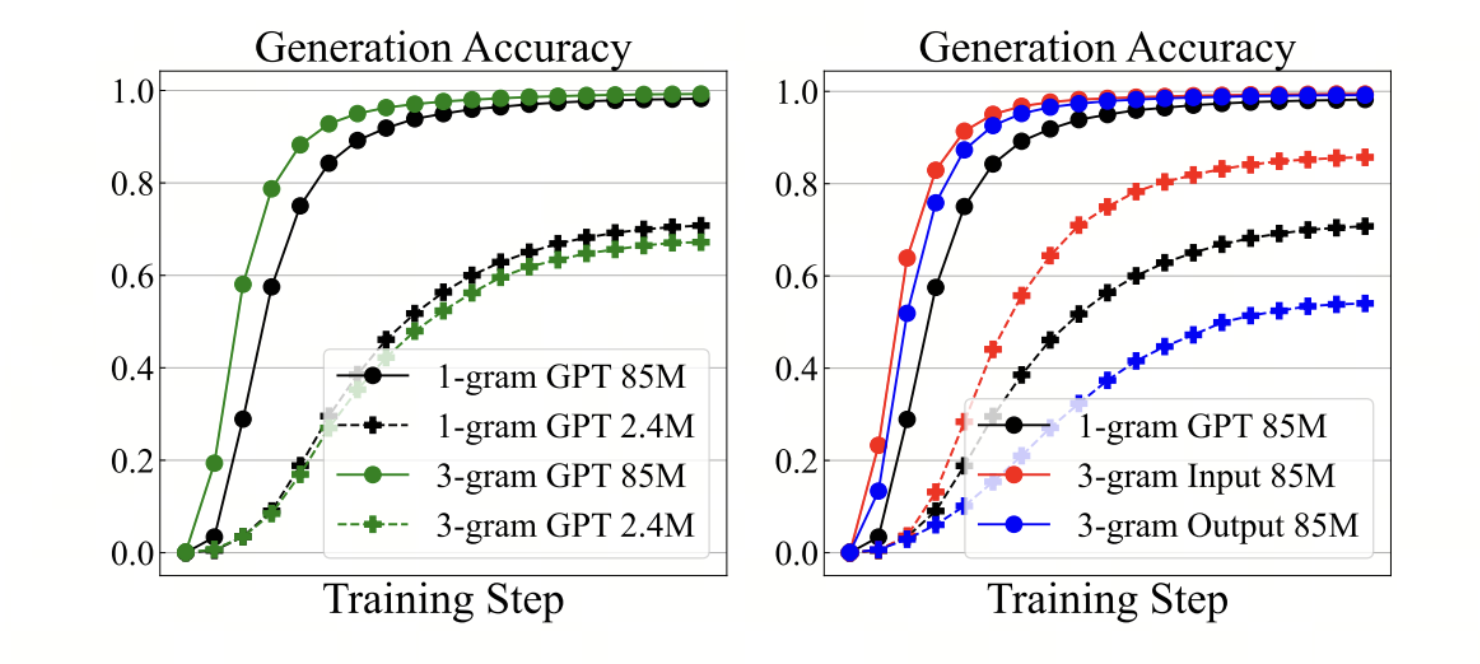
\includegraphics[width=0.9\linewidth,height=\textheight,keepaspectratio,alt={Input / Output Vocabulary 对不同规模模型的影响}]{assets/over-encoding-vocabulary.png}

\end{center}

Over Encoding（OE）发现，实际上是 \textbf{大 output vocabulary} 导致的。

这里有一个很直觉的解释：input vocabulary
增大，本质是在增强\textbf{上下文到 representation 的映射能力}；而 output
vocabulary
增大，则是在把预测问题变成更细粒度、更困难的分类任务。大模型有能力利用这种
supervision，小模型则容易 underfit。

从这个角度来讲，\textbf{input vocabulary 和 output vocabulary
不应该被绑定在一起 scaling}。

\subsubsection{Hierarchical N-gram 与 Feature
Hashing}\label{hierarchical-n-gram-ux4e0e-feature-hashing}

做法上，论文保留原来的 BPE token 序列不变，但把每个位置的输入 embedding
从``只查当前 token''，改成\textbf{同时查当前 token 及其历史 n-gram}。

例如，当前位置为 \(c\)，前两个 token 是 \(a,b\)，则构造：

\begin{itemize}
\tightlist
\item
  \textbf{1-gram}：\(c\)；
\item
  \textbf{2-gram}：\((b,c)\)；
\item
  \textbf{3-gram}：\((a,b,c)\)。
\end{itemize}

\begin{NotesFormula}

先用下面的函数，把每个固定长度的 n-gram 唯一编码成一个巨大整数：

\[
f(z_1,\ldots,z_n)=\sum_{j=1}^{n}z_j V^{j-1},
\]

\end{NotesFormula}

其中 \(V\) 是基础词表大小。由于理论上有 \(V^n\) 种组合，不可能真的建
\(V^n\) 行 embedding，作者使用 \textbf{feature hashing}，直接计算
\(f(\cdot)\bmod m\)，只查一个 \(m\) 行的表
\(E[f(\cdot)\bmod m]\)，允许不同 n-gram 碰撞到同一行。

\begin{NotesFormula}

所谓 \textbf{hierarchical n-gram}，就是不是只用
3-gram，而是在同一个位置同时加入 \(1+2+\cdots+n\)-gram embedding。例如：

\[
h_c=E_1[c]+E_2\!\left[f(b,c)\bmod m\right]
+E_3\!\left[f(a,b,c)\bmod m\right].
\]

\end{NotesFormula}

从而同时保留单 token、短局部组合和更长局部组合的信息。

\subsubsection{Sliced Low-Dimensional
Embeddings}\label{sliced-low-dimensional-embeddings}

\begin{NotesFormula}

进一步，对于每一种 n-gram，作者不是只建一个宽的 \(m\times d\)
表，而是使用 \textbf{sliced low-dimensional
embeddings}：把同样的参数预算拆成 \(k\) 个较窄的 \(m_i\times(d/k)\)
表，每次 lookup 出低维向量后，用
\(W_i\in\mathbb{R}^{(d/k)\times d_{\mathrm{model}}}\)
投影回模型维度，再相加：

\[
E_{\mathrm{slice}}(x)=\sum_{i=1}^{k}E_i[x\bmod m_i]W_i.
\]

\end{NotesFormula}

关键是这些 slice 的 \(m_i\) 故意设得略有不同，如
\(m,m+2,m+4\)。于是，同一个 n-gram 会得到
\(x\bmod m\)、\(x\bmod(m+2),\ldots\) 多组不同的 hash
地址：即使它在一个表里和别的 n-gram 撞车，也很难在所有表里同时撞车。

最终就是 \textbf{BPE embedding + 多层级 n-gram × 多个不同 hash view
的低维 embedding}，全部相加后送进原封不动的
Transformer。因此，增加的是大量稀疏 lookup 参数，而几乎不增加
Transformer 主干 FLOPs。

从上述流程也可以看出，OE 的 \textbf{hash 地址和稀疏查表只依赖 token
ID}，不需要等待 contextual hidden state，特别适合放到
CPU，甚至提前计算。查表后的 Linear 投影仍有矩阵运算，但 OE
参数虽然很大，每个 token 只访问极少几行。换个视角来说，这也是一种对
input embedding 的稀疏化。

\begin{Shaded}
\begin{Highlighting}[]
\NormalTok{2{-}gram (b,c)   {-}\textgreater{} hash\_i {-}\textgreater{} Emb\_i {-}\textgreater{} Linear\_i {-}\textgreater{} sum\_i {-}{-}+}
\NormalTok{3{-}gram (a,b,c) {-}\textgreater{} hash\_i {-}\textgreater{} Emb\_i {-}\textgreater{} Linear\_i {-}\textgreater{} sum\_i {-}{-}+{-}\textgreater{} SUM}
\NormalTok{1{-}gram c      {-}\textgreater{} Token Embedding {-}{-}{-}{-}{-}{-}{-}{-}{-}{-}{-}{-}{-}{-}{-}{-}{-}{-}{-}{-}{-}{-}{-}{-}+     |}
\NormalTok{                                                              v}
\NormalTok{                                                    Transformer {-}\textgreater{} LM Head}
\end{Highlighting}
\end{Shaded}

每条 n-gram 分支里的 \(i=1,\ldots,k\) 对应多个
slice；先在分支内求和，再与基础 token embedding 相加。

\clearpage

\subsection{二、Per-Layer
Embeddings（PLE）}\label{ux4e8cper-layer-embeddingsple}

Gemma 3n、Gemma 4 E2B / E4B 都使用了 \textbf{Per-Layer Embeddings}。

Motivation 为：\textbf{减少 backbone 做``静态记忆''的负担，用 memory
scaling 换 compute scaling}，不同深度可以学不同的 token
prior。前者也是后续 Engram 的 motivation。

\begin{NotesFormula}

做法上，除了普通 token embedding 之外，再给每个 token
在每一层都准备一份独立的低维 embedding，例如：

\[
\text{token}\times\text{layer}\;\longrightarrow\;\text{256-d vector}.
\]

\end{NotesFormula}

模型运行到第 \(m\) 层时，会取出这个 token 对应的第 \(m\) 层 PLE，用当前
contextual hidden state 乘 gate 矩阵，再过 GELU 产生一个
gate，选择性读取其中的信息，然后投影回 hidden dimension，加到 residual
stream。

它的本质可以理解为一种 \textbf{layer-specific token
memory}：让深层网络不必完全依赖前面几十层去保存原始 token
信息，而是每层都能直接访问一份针对该层专门学习的静态记忆。

这样可以用大量、稀疏访问的 embedding
参数提升模型容量，同时只增加较少的实际计算。

\subsection{三、Engram}\label{ux4e09engram}

\subsubsection{Motivation：Conditional
Memory}\label{motivationconditional-memory}

Engram 比较难得，是一篇在技术上和写作上都很棒的 paper，并且在吸取了 OE
与 PLE 的设计经验后进一步创新。我们来细读一下。

首先是 motivation 上，将大模型的计算分为：

\begin{enumerate}
\def\labelenumi{\arabic{enumi}.}
\item
  \textbf{动态、组合性的计算}：逻辑推理、数学推导、代码、长距离关系等，需要真正的深层
  block 计算。
\item
  \textbf{静态、局部、重复的模式}：人名、地名、固定短语、习语、常见局部组合等，本质上更类似``看到
  key，取出 value''，并不需要很深的计算来获取这类 factual knowledge。
\end{enumerate}

\textbf{在此之外，作者还有另外更大的野心：希望找到第二个 sparsity 轴，即
Conditional Memory；以及在 dense compute 和 MoE experts 之外，找到 LLM
的第三种容量 scaling 方式：增加静态、稀疏访问的 memory。}

\subsubsection{从 N-gram Lookup 到 Residual
Injection}\label{ux4ece-n-gram-lookup-ux5230-residual-injection}

\begin{center}

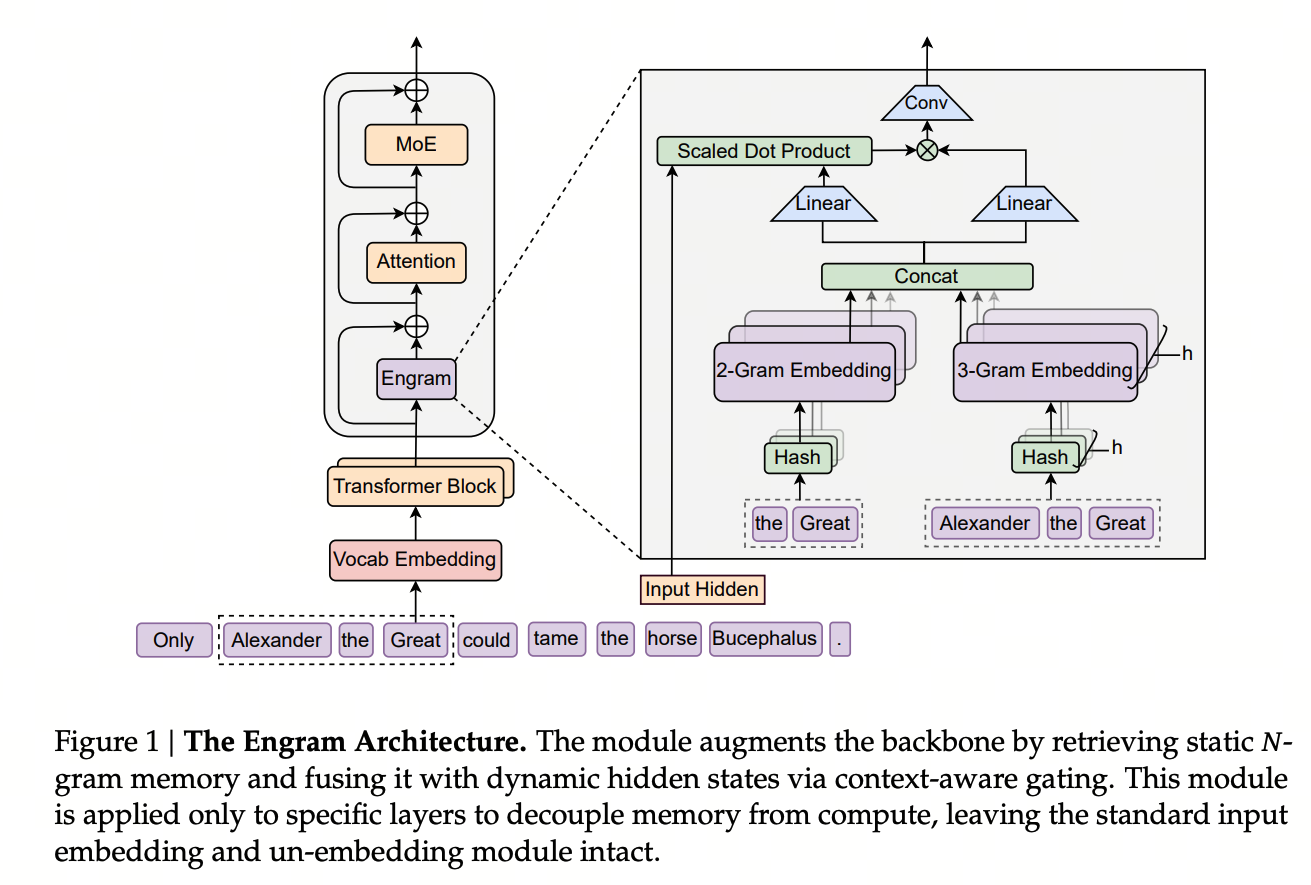
\includegraphics[width=0.9\linewidth,height=\textheight,keepaspectratio,alt={Engram 架构与条件记忆读取}]{assets/engram-architecture.png}

\end{center}

因为大模型 tokenizer 中，许多\textbf{文本形式近似等价的 token
却拥有完全不同的 ID}，例如大小写差异、是否带前导空格等，Engram 首先对
token 做 \textbf{canonicalization}，将这些变体映射到更统一的表示空间。

\begin{NotesFormula}

随后，在当前位置构造 2-gram、3-gram 等局部短语，并通过多个独立 hash
函数映射到超大的 embedding table 中进行查表：

\[
e_t=\operatorname{Concat}\!\left(
\left\{E_{n,k}[\phi_{n,k}(g_{t,n})]\right\}_{n,k}
\right).
\]

\end{NotesFormula}

\begin{NotesFormula}

查出的 memory \(e_t\) 经过共享的 Value projection \(W_V\)，得到：

\[
v_t=W_Ve_t.
\]

\end{NotesFormula}

\begin{NotesFormula}

在 mHC 中，同一层的多个 residual stream 共享这份 memory 和
\(W_V\)，但每个 branch \(m\) 拥有独立的 \(W_K^{(m)}\)。模型利用当前
branch 的 hidden state \(h_t^{(m)}\) 与 memory key 计算
\textbf{context-aware gate}：

\[
\alpha_t^{(m)}=\sigma\!\left(
\frac{
\operatorname{RMSNorm}(h_t^{(m)})^{\top}
\operatorname{RMSNorm}(W_K^{(m)}e_t)
}{\sqrt{d}}
\right).
\]

\end{NotesFormula}

\begin{NotesFormula}

从而得到该 branch 实际读取的 memory：

\[
\tilde v_t^{(m)}=\alpha_t^{(m)}v_t.
\]

\end{NotesFormula}

\begin{NotesFormula}

最后，原文中声称是为了进一步扩大局部感受野并增强非线性，在 gated memory
序列 \(\tilde V\) 上加入一个轻量的 \textbf{short depthwise causal
convolution}：

\[
Y=\operatorname{SiLU}\!\left(
\operatorname{Conv1D}\!\left(\operatorname{RMSNorm}(\tilde V)\right)
\right)+\tilde V.
\]

\end{NotesFormula}

（这玩意儿我很存疑。）

最终 \(Y\) 再写回对应的 residual
stream。整体上就是：\textbf{canonicalization → N-gram hash lookup →
context-aware gated retrieval → local causal convolution refinement →
residual injection}。

\subsubsection{Infra：Host Memory 与
Prefetch}\label{infrahost-memory-ux4e0e-prefetch}

与 OE 同理，由于 hash 地址只依赖 token ID，memory 可以提前在 CPU / Host
DRAM 查表并异步搬到
GPU，与前层计算重叠。因此，可以把参数规模扩得很大，而每个 token 的
lookup 数量保持不变；投影、gate 与卷积仍有少量计算开销。

\begin{center}

\pandocbounded{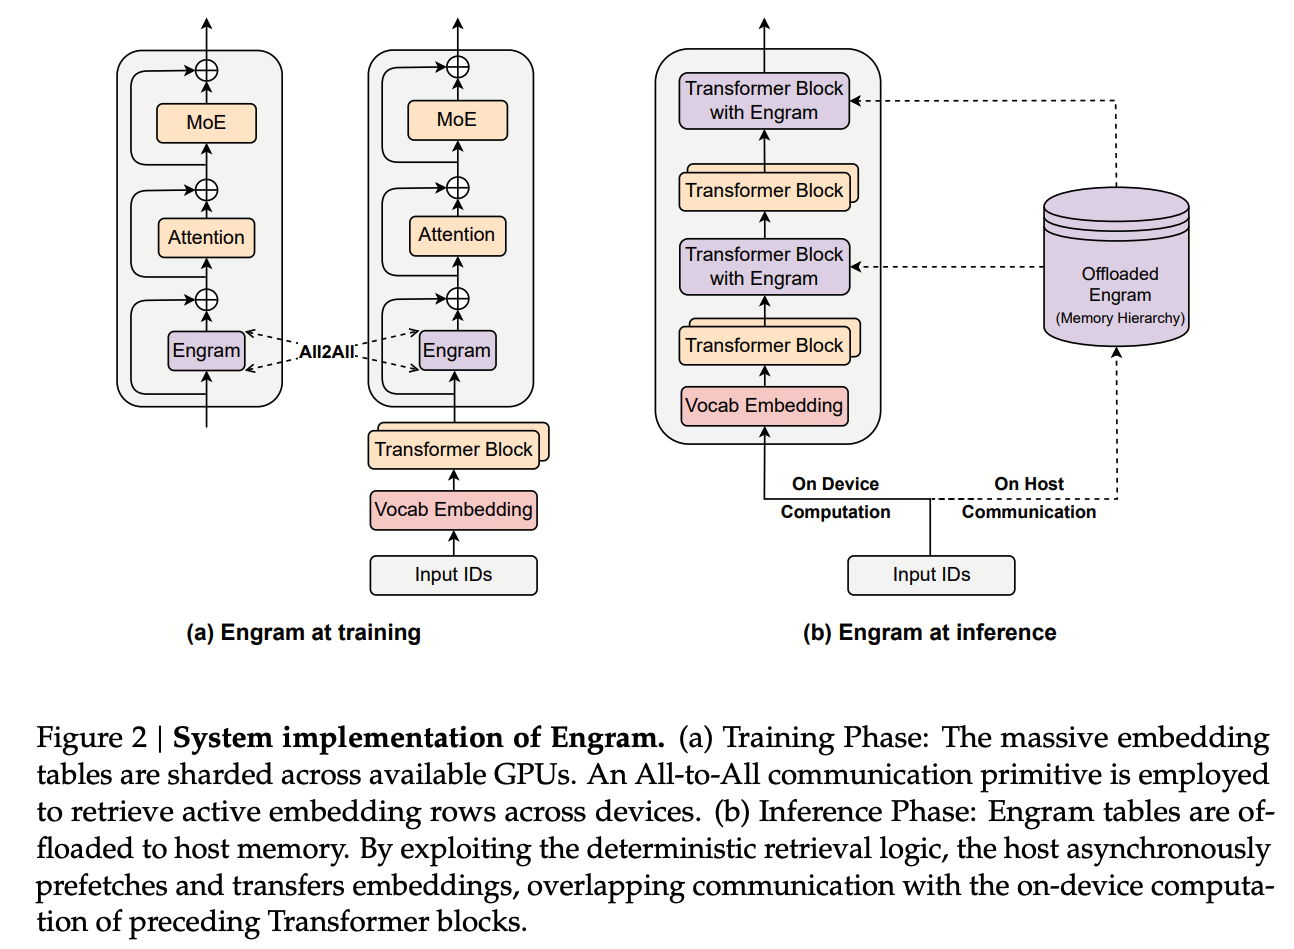
\includegraphics[keepaspectratio,alt={Engram 的训练与推理系统实现}]{assets/engram-system.png}}

\end{center}

\clearpage

\subsubsection{有趣的实验问题与结论}\label{ux6709ux8da3ux7684ux5b9eux9a8cux95eeux9898ux4e0eux7ed3ux8bba}

实验结果就无需多言。接着，我们看看文章里有哪些有趣的实验问题与结论。

\begin{enumerate}
\def\labelenumi{\arabic{enumi}.}
\item
  \textbf{固定预算下，MoE 和 Engram 的参数怎么分？}

  固定总参数和激活参数，只改变 sparse budget 在 MoE 与 Engram
  之间的分配。结果呈明显 U 型：纯 MoE 不是最优，大约 \textbf{75\%-80\%
  给 MoE、20\%-25\% 给 Engram} 效果最好。
\item
  \textbf{Engram 可以 scale 吗？}

  可以。固定 backbone，只不断扩大 Engram table，validation loss
  持续下降，并呈较稳定的 scaling 趋势。更 nice 的是：memory table
  可以变得很大，但每个 token 只查固定数量的
  row，因此参数规模增长并不会同比增加 FLOPs。所以，memory size
  可以成为独立于模型计算量之外的新 scaling axis。
\item
  \textbf{N-gram memory 能改善 reasoning 吗？}

  可以！虽然 Engram
  本身不是在``做推理''，但有了它，也许前几层不必花计算重新组合静态实体和短语，因此能更早进入高层语义处理。LogitLens
  和 CKA 显示，Engram 模型在更浅层就能形成接近 baseline
  更深层的表示，因此作者称其提升了 \textbf{effective
  depth}：把更多真正的 Transformer 深度留给组合推理、数学和代码。
\item
  \textbf{Engram 能改善长上下文吗？}

  可以！普通 Attention 不仅要处理长程依赖，还要承担大量局部 pattern
  建模；Engram 把一部分 local dependency 直接交给 memory
  lookup。这样，Attention capacity 可以更多用于 global
  dependency。（写到这里，不禁再次让我想到 Zeyuan 的语言模型物理学。）
\item
  \textbf{Engram 应该放在哪一层？哪些组件真正有用？}

  这也是一个需要 trade-off 的事情。直觉来想，太早时 hidden state 缺少
  context，可能 gate
  不准；太晚又已经浪费了前层计算。文章实验发现，在第二层放置最好，把预算拆成多个
  Engram、分布在不同深度，还能进一步提升。

  消融上，\textbf{context-aware gate、tokenizer compression、mHC
  branch-specific fusion} 最关键；Short Causal Conv 只有小幅增益（于是
  DS4.1 干脆删了）。
\item
  \textbf{Engram 到底学了什么？}

  关闭 Engram
  后，事实知识类任务性能大幅下降，而阅读理解保留得更多。这说明模型自然形成了功能分工：Engram
  更偏向存储实体、事实、固定短语等静态 parametric knowledge；Transformer
  backbone 更偏向上下文处理、组合与推理。
\end{enumerate}

当然，以上结论都是在小 size 模型上做的。在现在的发版模型中，具体 Engram
的配置也有了一些变化。

\clearpage

\subsection{四、Qwen3.8 Flash Next
的消融}\label{ux56dbqwen3.8-flash-next-ux7684ux6d88ux878d}

在这里，我简单提下 Qwen3.8 Flash Next 中的消融结论。

\begin{center}

\pandocbounded{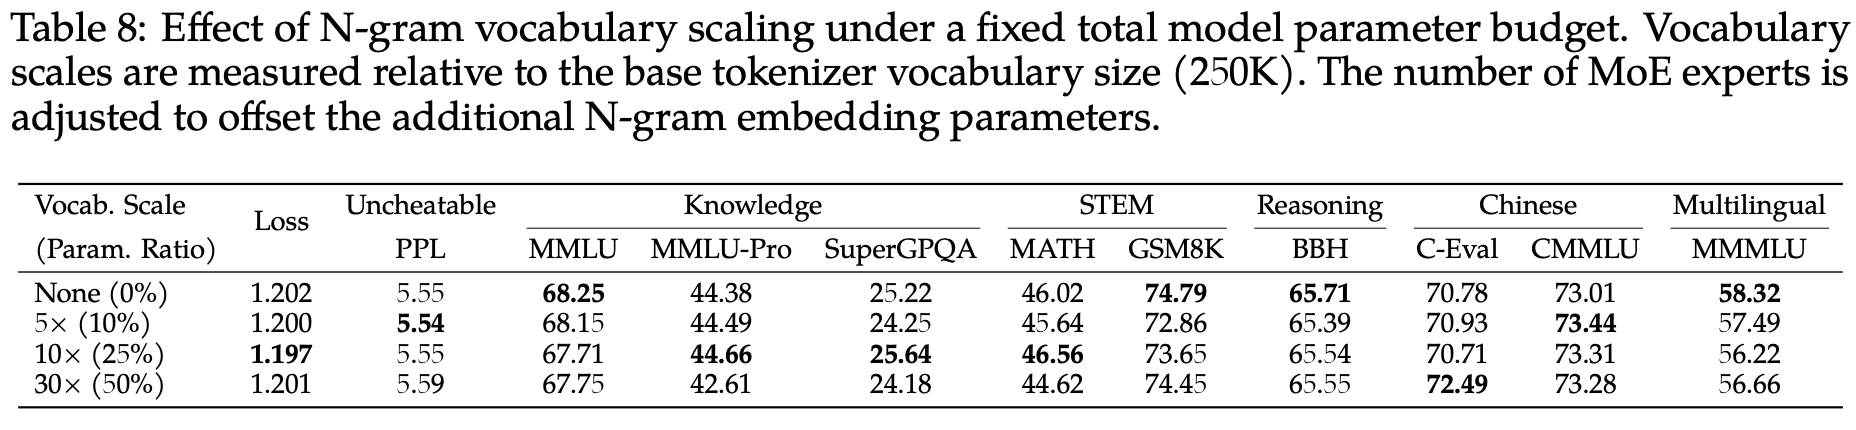
\includegraphics[keepaspectratio,alt={固定总参数预算下的 N-gram 词表扩展}]{assets/qwen-fixed-budget.png}}

\end{center}

\begin{enumerate}
\def\labelenumi{\arabic{enumi}.}
\item
  \textbf{N-gram 层数放置。}
  浅层总体较强，但中层、深层也有竞争力；把固定参数预算拆成两层并没有稳定收益。因此，最终选择\textbf{只放
  Layer 2}。放在 Layer 2，可以在计算 Layer 1 时，从 host memory 提前
  prefetch N-gram embedding。
\item
  \textbf{固定总参数预算。} 约 25\% 参数给 N-gram 时，training loss
  最好，但 downstream 评估上并没有对应的 25\% 最优点。
\item
  \textbf{固定 backbone，额外增加 N-gram 参数。} 从 loss 上来看，N-gram
  可以持续 scale。但是，``\textbf{loss 越低 ≠ downstream
  越好}''：reasoning benchmark 到一定规模之后会持平，甚至下降。
\item
  \textbf{中文 benchmark。} N-gram 对中文 benchmark（如 C-Eval 和
  CMMLU）的 scaling 特别稳定。
\end{enumerate}

\begin{center}

\pandocbounded{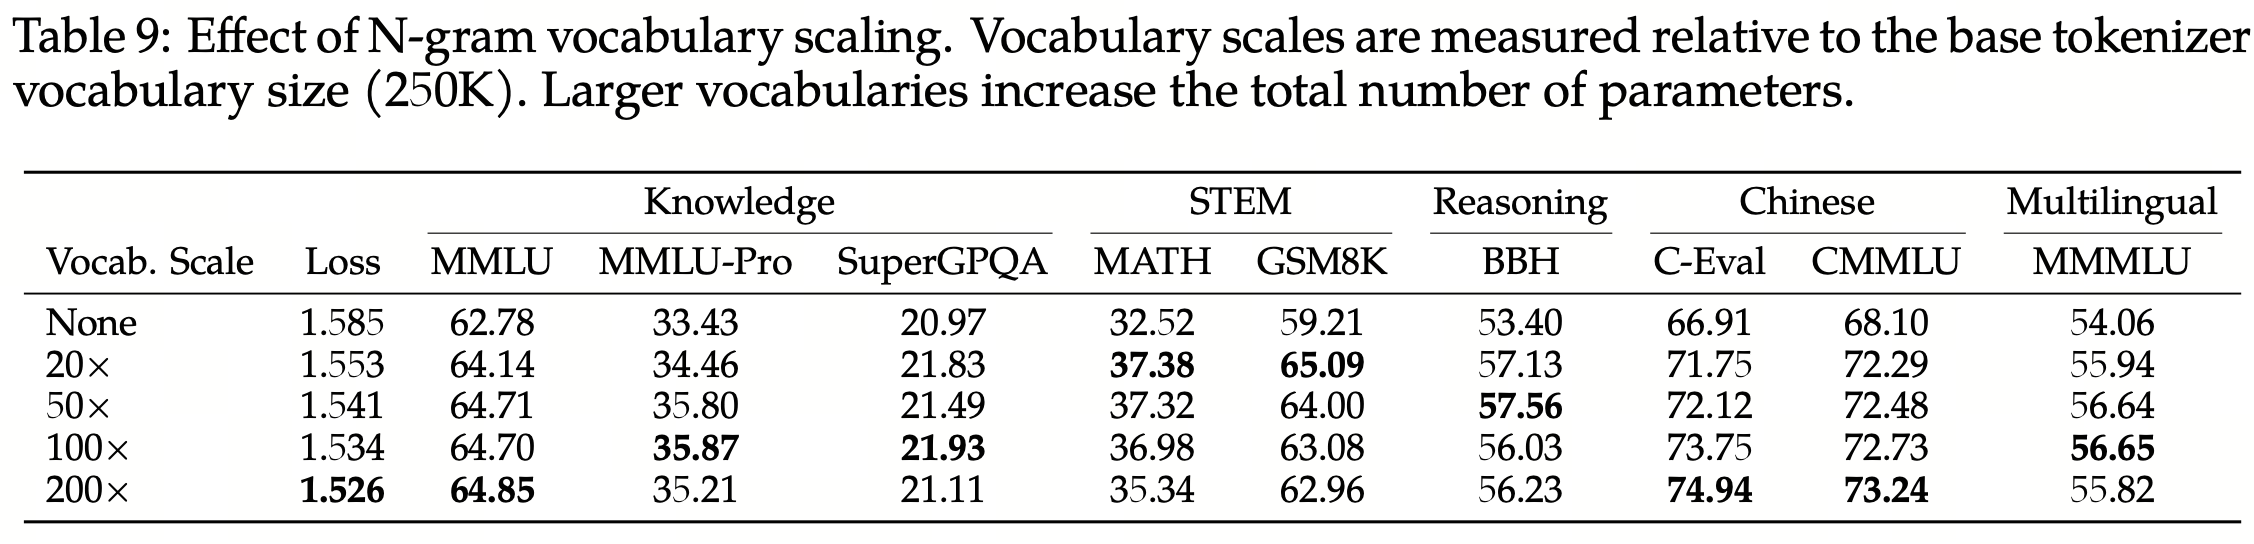
\includegraphics[keepaspectratio,alt={固定 backbone 下增加 N-gram 参数的 scaling 结果}]{assets/qwen-memory-scaling.png}}

\end{center}

此外，LongCat-2.0
的选择也略有不同，在这里我不再赘述，感兴趣的可以去看他们的技术报告。

\end{document}
